% ------------------------------------------------------------------------------
% 8.2. IMPLEMENTACIÓN DE LA ARQUITECTURA DEL SUBSISTEMA
% ------------------------------------------------------------------------------
\wfa{\wn{8}.2. Implementación de la Arquitectura del Subsistema}\label{sec:cap8_arquitectura_subsistema}

Cada subsistema sigue la misma arquitectura en tres capas, que corresponde a la organización por \textit{features} del código. La capa de cliente contiene las pantallas del panel web (una carpeta por \textit{feature} en React) y, cuando el caso de uso lo requiere, las pantallas y servicios de la aplicación móvil. La capa de servicio y negocio está en el paquete \texttt{com.comedoruagrm.backend.features} de Spring Boot: los controladores REST validan la entrada y delegan en servicios; los servicios contienen la lógica, las transacciones y la auditoría; y los repositorios, interfaces de Spring Data JPA o consultas SQL directas, acceden a la base de datos. La capa de base de datos corresponde a las tablas de PostgreSQL de cada paquete funcional. Las flechas de los diagramas indican dependencia de uso y se obtuvieron de las dependencias inyectadas en el código; para no recargar los diagramas, no se dibujan las lecturas de apoyo a tablas de otros subsistemas.


\wfb{\wn{8}.2.1. Implementación de la Arquitectura del Subsistema Cuentas y Acceso}\label{sec:cap8_sub_p1}

Este subsistema agrupa los casos de uso CU01, CU14, CU15.

Gestiona las cuentas del sistema: registro e inicio de sesión con JWT propio (token de acceso de 15 minutos y \textit{refresh token} de 7 días, enviados en cookies \texttt{HttpOnly} en la web y como \textit{Bearer} en móvil), recuperación y cambio de contraseña mediante un enlace enviado por correo, perfil del usuario y administración de las cuentas del personal y sus roles. Los controladores delegan en los servicios del subsistema; la sesión se guarda en la tabla \texttt{sesion} solo como hash del \textit{refresh token}.

La Figura~\ref{fig:impl_p1} presenta el diagrama de componentes del subsistema. Sus componentes son los siguientes:

\begin{itemize}
\item \textbf{Cliente web:} \texttt{LoginScreen}, \texttt{RegistroScreen}, \texttt{RecuperarContrasenaScreen}, \texttt{RestablecerContrasenaScreen}, \texttt{PerfilScreen}, \texttt{UsuariosPersonalScreen}.
\item \textbf{Cliente móvil:} \texttt{login\_screen}, \texttt{registro\_screen}, \texttt{recuperar\_contrasena\_screen}, \texttt{perfil\_screen}.
\item \textbf{Controladores:} \texttt{AuthController}, \texttt{UsuarioController}, \texttt{PerfilController}, \texttt{CarreraController}.
\item \textbf{Servicios:} \texttt{AuthService}, \texttt{SesionService}, \texttt{RestablecimientoContrasenaService}, \texttt{CorreoRestablecimientoService}, \texttt{UsuarioService}, \texttt{UsuarioPersonalService}, \texttt{PerfilService}, \texttt{CarreraService}.
\item \textbf{Repositorios:} \texttt{SesionRepository}, \texttt{UsuarioRepository}, \texttt{PostulanteRepository}, \texttt{RolRepository}, \texttt{CarreraRepository}.
\item \textbf{Tablas:} \texttt{sesion}, \texttt{usuario}, \texttt{postulante}, \texttt{rol}, \texttt{carrera}.
\item \textbf{Componentes externos:} Servicio de correo (SMTP).
\end{itemize}

\begin{landscape}
\begin{figure}[p]
\caption{Diagrama de Componentes de la Implementación de la Arquitectura del Subsistema Cuentas y Acceso}
\label{fig:impl_p1}
\centering
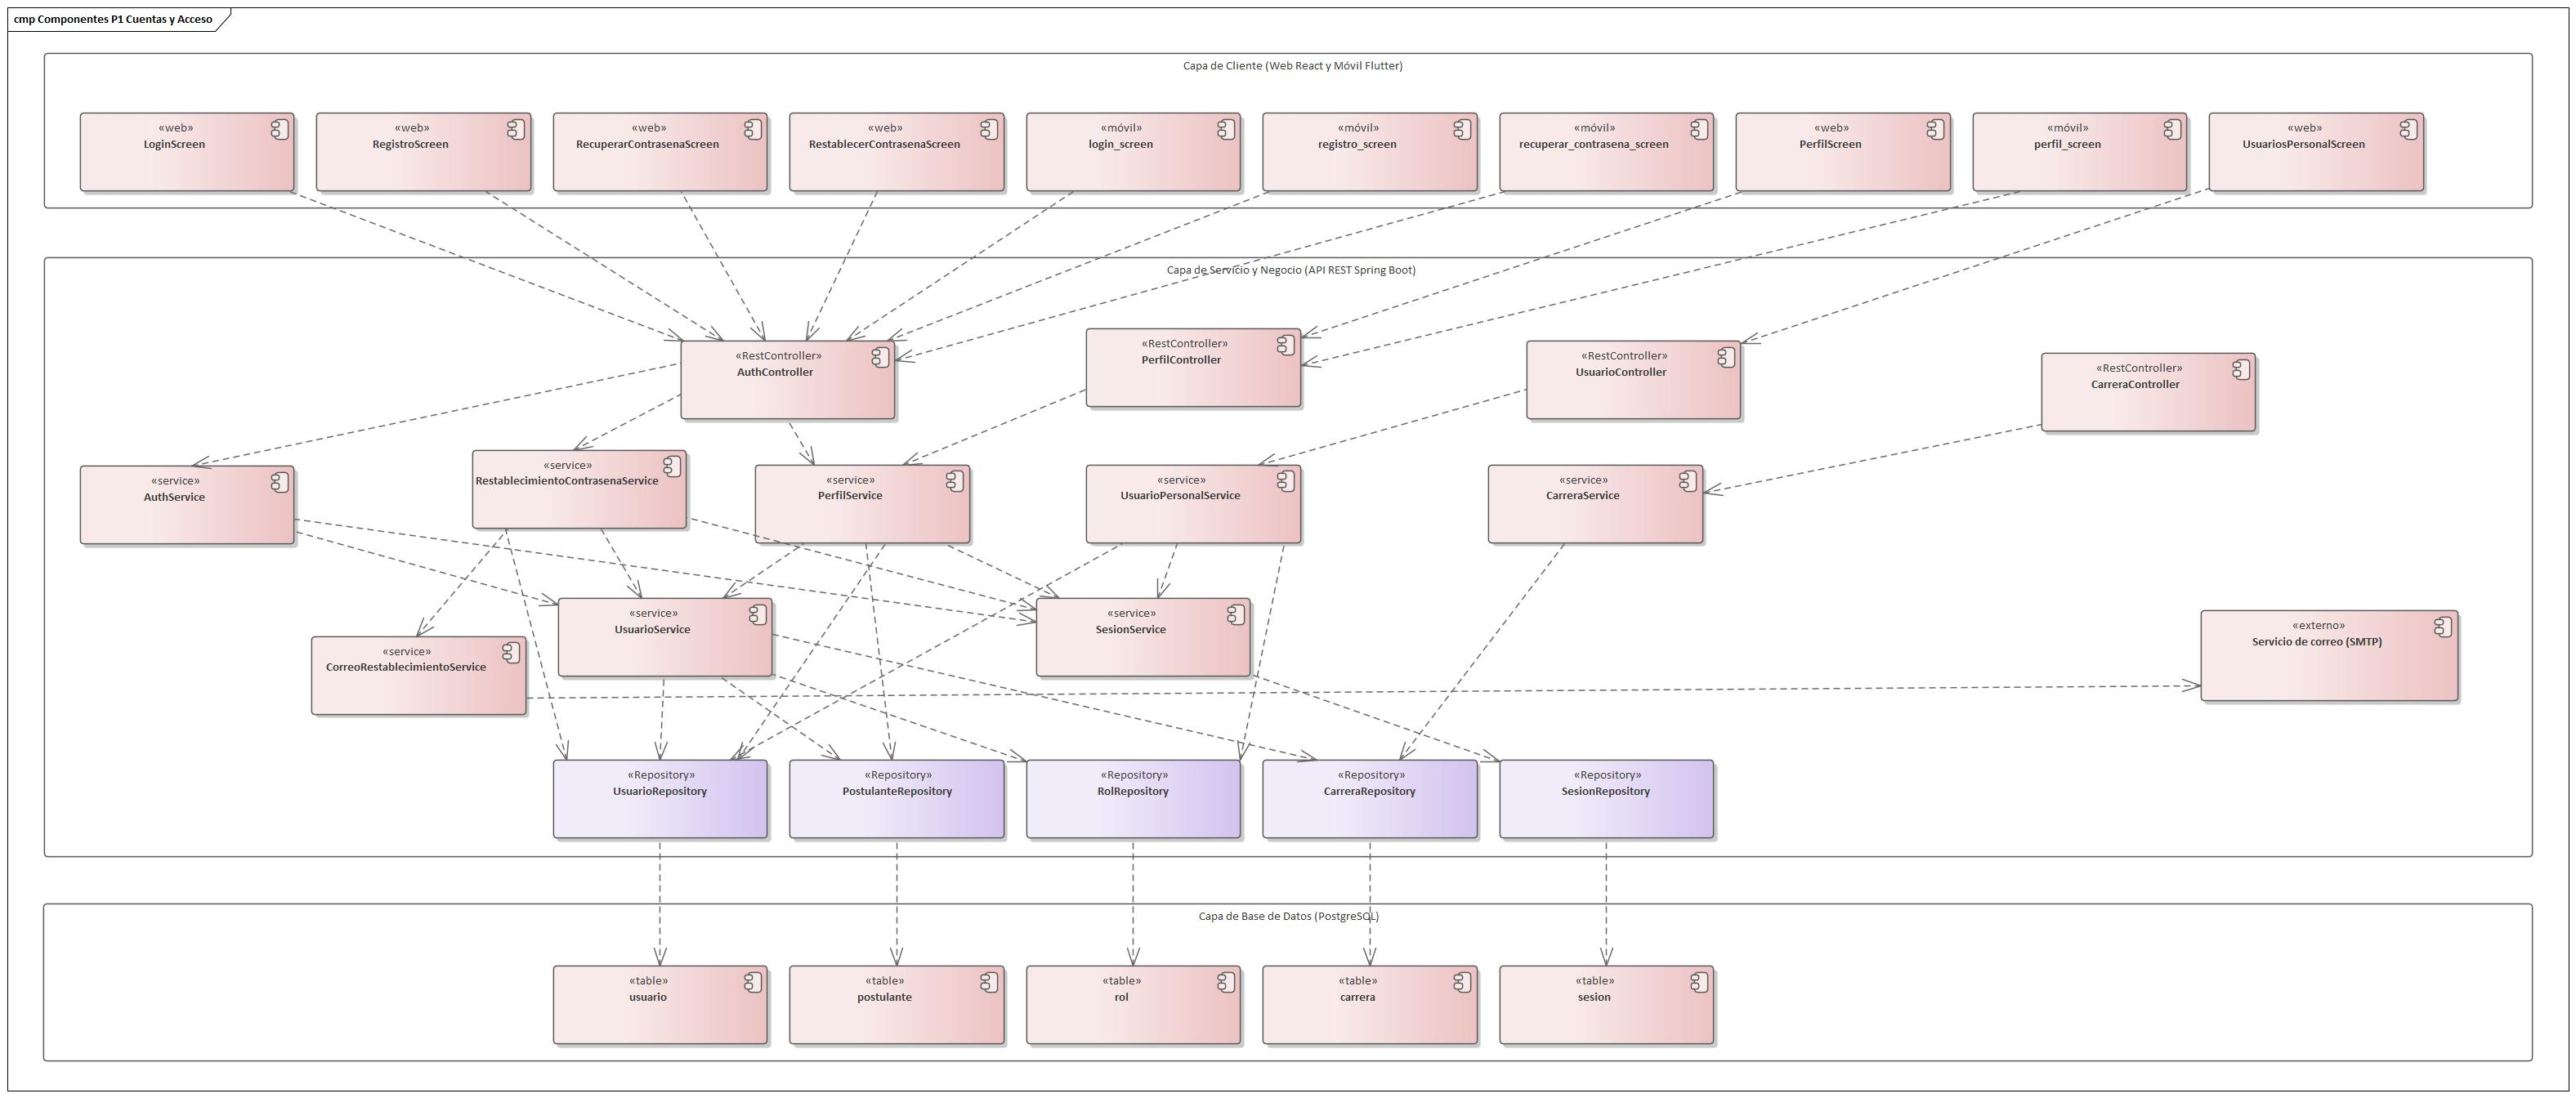
\includegraphics[width=\linewidth,height=0.8\textheight,keepaspectratio]{images/148_Componentes_P1_Cuentas_y_Acceso.jpg}

\smallskip
\noindent\raggedright\textit{Nota.} Elaboración propia.
\end{figure}
\end{landscape}


\wfb{\wn{8}.2.2. Implementación de la Arquitectura del Subsistema Convocatoria y Postulación}\label{sec:cap8_sub_p2}

Este subsistema agrupa los casos de uso CU13, CU02, CU16, CU17, CU18, CU04.

Cubre la apertura y cierre de convocatorias y gestiones académicas, y la postulación del estudiante: guardar el borrador, adjuntar documentos (almacenados en MinIO), validar elegibilidad y duplicados, enviar la postulación y consultar su estado. \texttt{CierreAutomaticoConvocatoriasJob} cierra las convocatorias vencidas. Al enviar la postulación, \texttt{EnvioPostulacionService} dispara la precalificación del subsistema de preselección con IA.

La Figura~\ref{fig:impl_p2} presenta el diagrama de componentes del subsistema. Sus componentes son los siguientes:

\begin{itemize}
\item \textbf{Cliente web:} \texttt{ConvocatoriasScreen}, \texttt{GestionesAcademicasScreen}, \texttt{PostularScreen}, \texttt{MisPostulacionesScreen}, \texttt{DetallePostulacionScreen}, \texttt{DocumentosPostulacionScreen}.
\item \textbf{Cliente móvil:} \texttt{postular\_screen}, \texttt{detalle\_postulacion\_screen}, \texttt{documentos\_postulacion\_screen}, \texttt{revisar\_documento\_screen}.
\item \textbf{Controladores:} \texttt{ConvocatoriaController}, \texttt{GestionAcademicaController}, \texttt{TipoDocumentoController}, \texttt{EnvioPostulacionController}, \texttt{BorradorPostulacionController}, \texttt{DocumentosPostulacionController}, \texttt{MisPostulacionesController}.
\item \textbf{Servicios:} \texttt{ConvocatoriaService}, \texttt{ConvocatoriaEstadoService}, \texttt{GestionAcademicaService}, \texttt{TipoDocumentoService}, \texttt{DocumentosConvocatoriaService}, \texttt{CierreAutomaticoConvocatoriasJob}, \texttt{EnvioPostulacionService}, \texttt{BorradorPostulacionService}, \texttt{DocumentosPostulacionService}, \texttt{ValidacionPostulacionService}, \texttt{MisPostulacionesService}.
\item \textbf{Repositorios:} \texttt{ConvocatoriaRepository}, \texttt{ConvocatoriaDocumentoRepository}, \texttt{GestionAcademicaRepository}, \texttt{TipoDocumentoRepository}, \texttt{PostulacionRepository}, \texttt{DocumentoAdjuntoRepository}, \texttt{PostulacionHistorialRepository}.
\item \textbf{Tablas:} \texttt{convocatoria}, \texttt{convocatoria\_documento}, \texttt{gestion\_academica}, \texttt{tipo\_documento}, \texttt{postulacion}, \texttt{documento\_adjunto}, \texttt{postulacion\_historial}.
\item \textbf{Componentes externos:} MinIO (archivos), Módulo de IA (FastAPI).
\end{itemize}

\begin{landscape}
\begin{figure}[p]
\caption{Diagrama de Componentes de la Implementación de la Arquitectura del Subsistema Convocatoria y Postulación}
\label{fig:impl_p2}
\centering
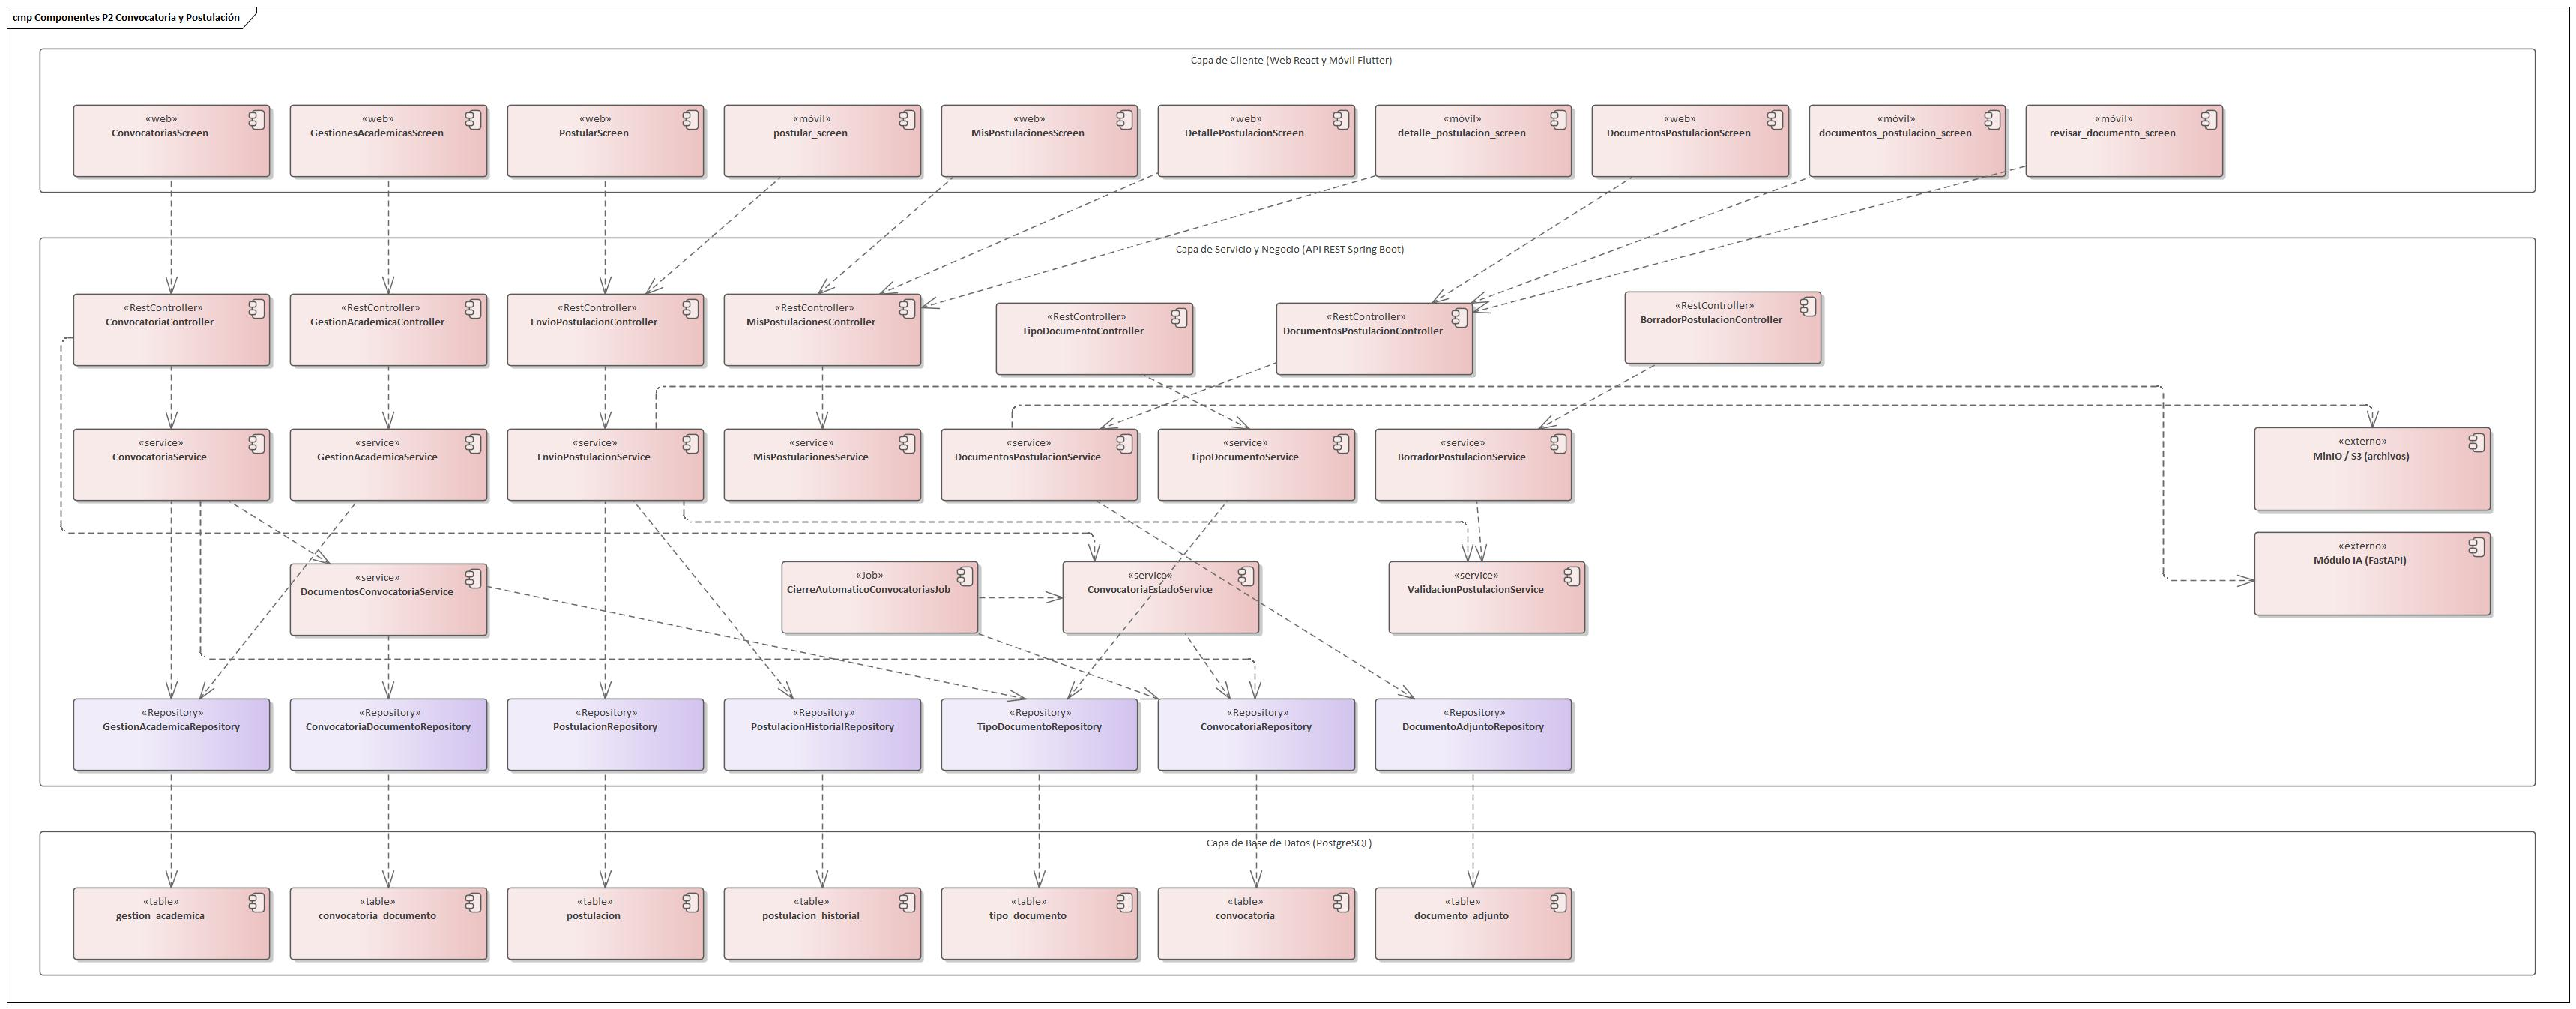
\includegraphics[width=\linewidth,height=0.8\textheight,keepaspectratio]{images/149_Componentes_P2_Convocatoria_y_Postulacion.jpg}

\smallskip
\noindent\raggedright\textit{Nota.} Elaboración propia.
\end{figure}
\end{landscape}


\wfb{\wn{8}.2.3. Implementación de la Arquitectura del Subsistema Preselección con IA}\label{sec:cap8_sub_p3}

Este subsistema agrupa los casos de uso CU03, CU26.

Calcula el puntaje de vulnerabilidad de cada postulación y permite a la DUBSS parametrizar el modelo y reprocesar los puntajes. \texttt{PrecalificacionClient} es la interfaz que abstrae al módulo de IA e \texttt{IaHttpPrecalificacionClient} la implementa llamando por HTTP interno a \texttt{POST /api/v1/puntaje} del módulo \texttt{comedor-uagrm-ia} (FastAPI); \texttt{PrecalificacionReintentoJob} reintenta las precalificaciones que fallaron. Los repositorios \texttt{ModeloPreseleccionConsultaRepository} y \texttt{ReprocesamientoConsultaRepository} acceden con SQL directo a \texttt{parametro\_modelo} y \texttt{lote\_reprocesamiento}.

La Figura~\ref{fig:impl_p3} presenta el diagrama de componentes del subsistema. Sus componentes son los siguientes:

\begin{itemize}
\item \textbf{Cliente web:} \texttt{PrecalificacionScreen}, \texttt{ParametrosModeloScreen}.
\item \textbf{Controladores:} \texttt{PrecalificacionController}, \texttt{ModeloPreseleccionController}, \texttt{ReprocesamientoController}.
\item \textbf{Servicios:} \texttt{PrecalificacionService}, \texttt{PrecalificacionDetalleService}, \texttt{IaHttpPrecalificacionClient}, \texttt{PrecalificacionReintentoJob}, \texttt{ModeloPreseleccionService}, \texttt{ReprocesamientoService}, \texttt{ReprocesamientoEjecucionService}.
\item \textbf{Repositorios:} \texttt{ModeloPreseleccionRepository}, \texttt{ModeloPreseleccionConsultaRepository}, \texttt{PuntajePostulacionRepository}, \texttt{ReprocesamientoConsultaRepository}.
\item \textbf{Tablas:} \texttt{modelo\_preseleccion}, \texttt{parametro\_modelo}, \texttt{puntaje\_postulacion}, \texttt{lote\_reprocesamiento}.
\item \textbf{Componentes externos:} Módulo de IA (FastAPI).
\end{itemize}

\begin{landscape}
\begin{figure}[p]
\caption{Diagrama de Componentes de la Implementación de la Arquitectura del Subsistema Preselección con IA}
\label{fig:impl_p3}
\centering
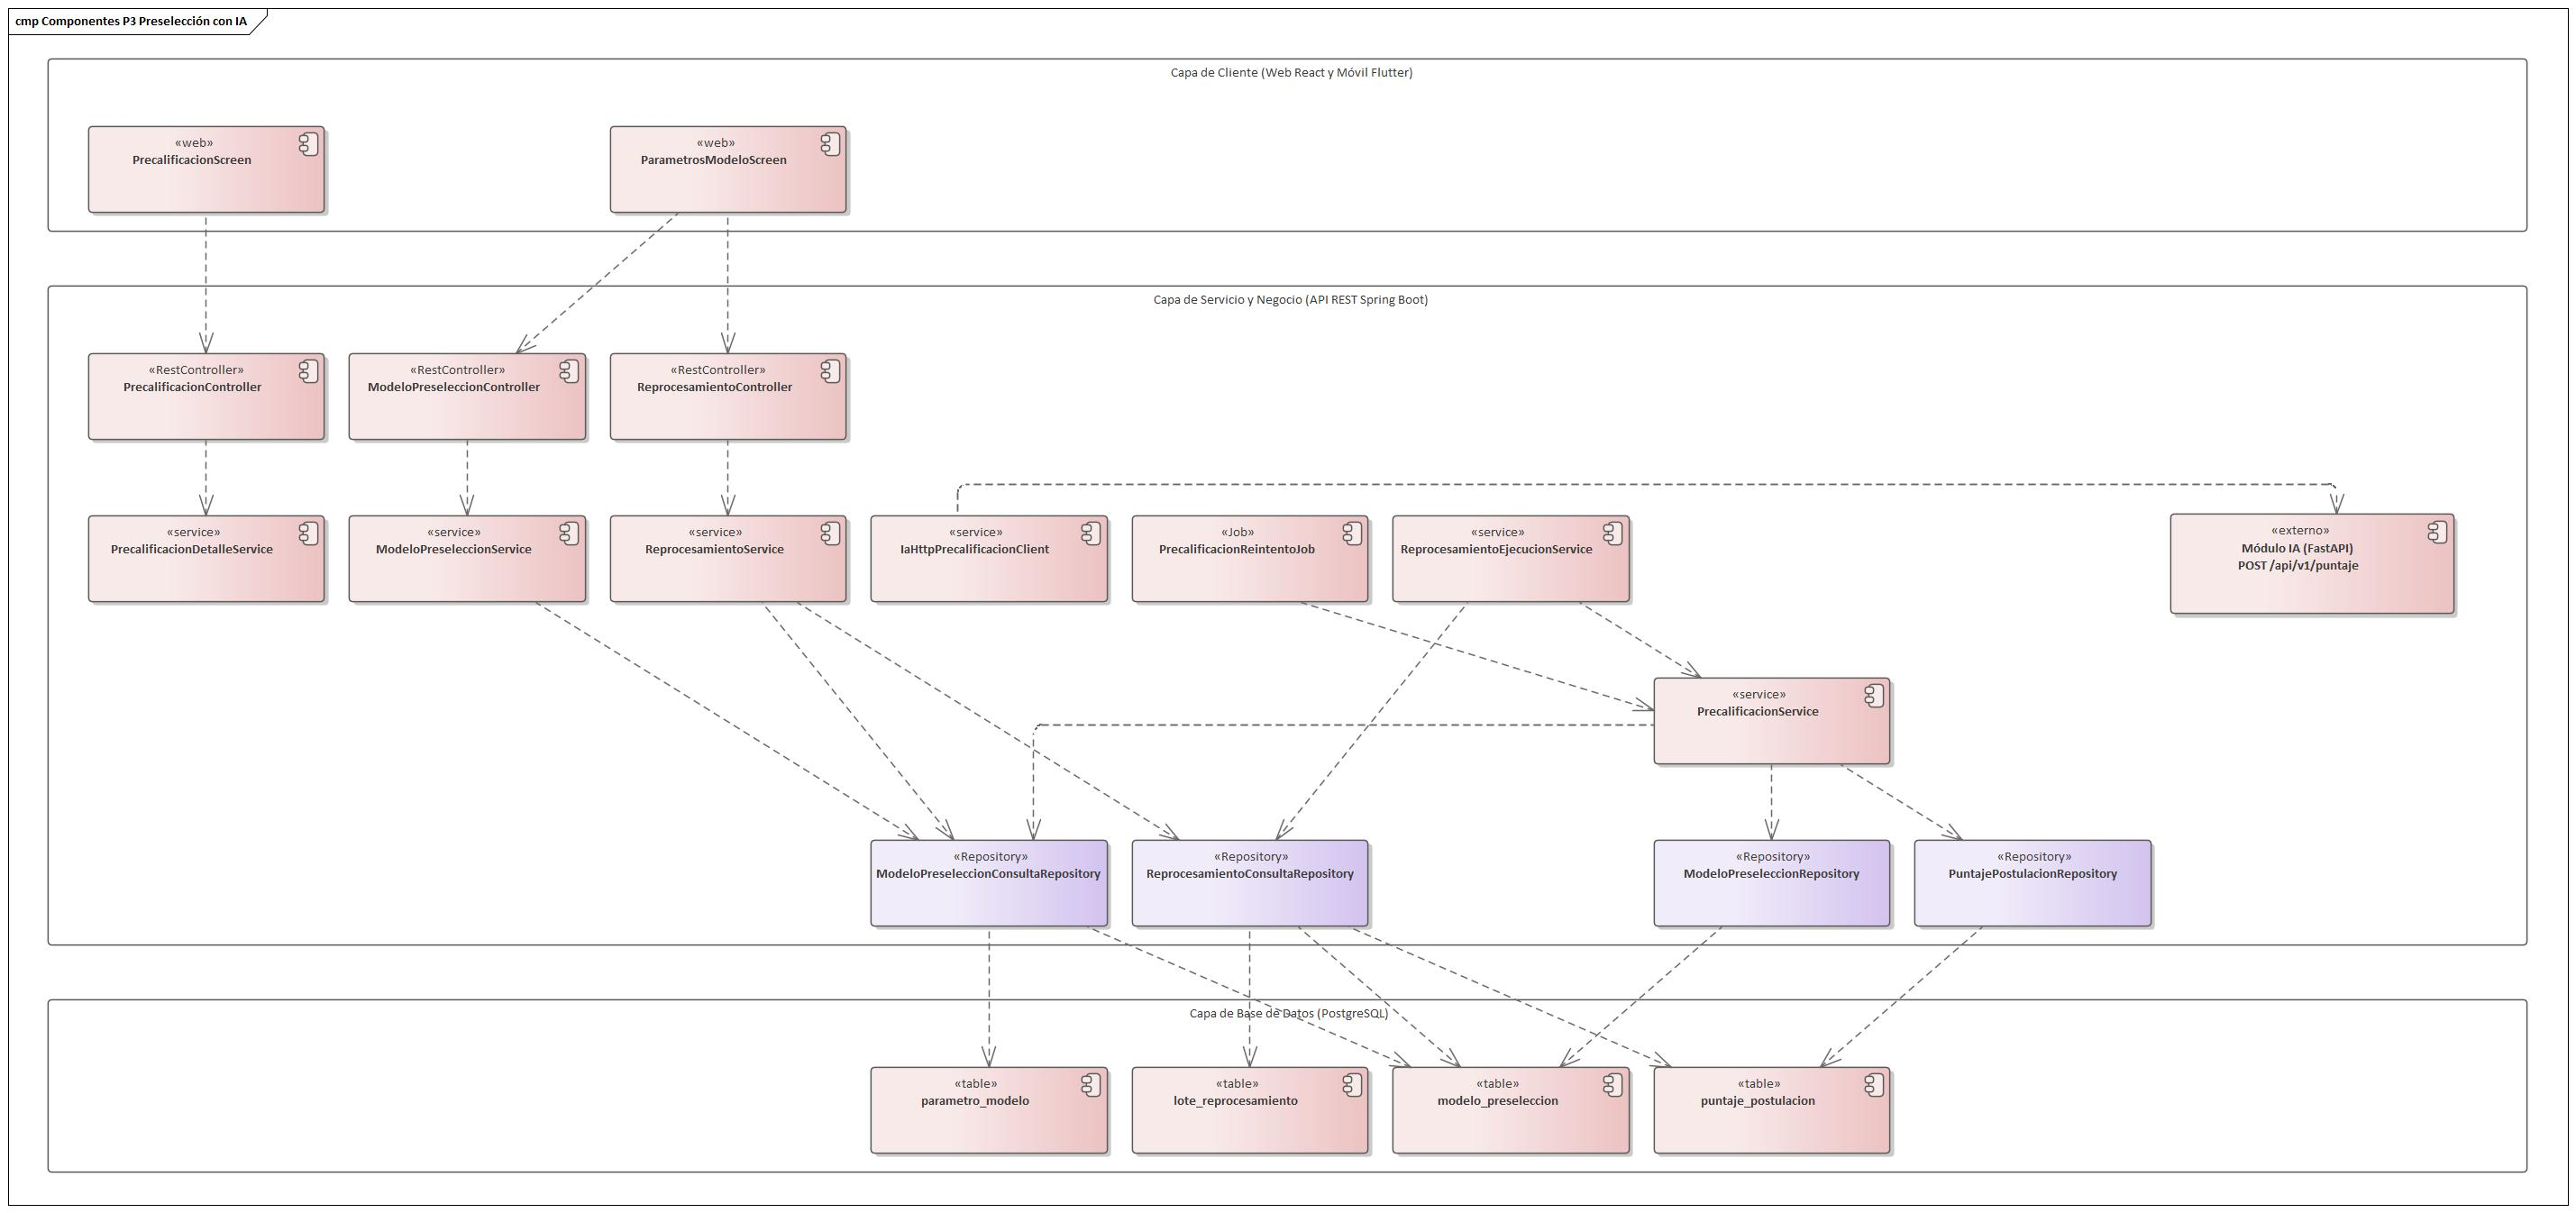
\includegraphics[width=\linewidth,height=0.8\textheight,keepaspectratio]{images/150_Componentes_P3_Preseleccion_IA.jpg}

\smallskip
\noindent\raggedright\textit{Nota.} Elaboración propia.
\end{figure}
\end{landscape}


\wfb{\wn{8}.2.4. Implementación de la Arquitectura del Subsistema Auditoría y Adjudicación}\label{sec:cap8_sub_p4}

Este subsistema agrupa los casos de uso CU05, CU06, CU07, CU08, CU19, CU20, CU21, CU22 y CU-EXTRA-01.

Concentra el proceso de la DUBSS sobre las postulaciones mejor puntuadas: lista priorizada, selección y notificación de finalistas, auditoría del expediente, devolución, archivo o rechazo, adjudicación, acta de adjudicación en PDF, comunicados y publicación de resultados. También contiene el servicio transversal de notificaciones (bandeja, correo y \textit{push} con Firebase Cloud Messaging) y el registro de dispositivos móviles.

La Figura~\ref{fig:impl_p4} presenta el diagrama de componentes del subsistema. Sus componentes son los siguientes:

\begin{itemize}
\item \textbf{Cliente web:} \texttt{ListaPriorizadaScreen}, \texttt{FinalistasScreen}, \texttt{ExpedienteScreen}, \texttt{AdjudicacionScreen}, \texttt{ActasScreen}, \texttt{PublicarResultadosScreen}, \texttt{ResultadosScreen}.
\item \textbf{Cliente móvil:} \texttt{firebase\_push\_service}.
\item \textbf{Controladores:} \texttt{ListaPriorizadaController}, \texttt{SeleccionFinalistasController}, \texttt{FinalistaController}, \texttt{ExpedienteController}, \texttt{DevolucionController}, \texttt{CierrePostulacionController}, \texttt{AdjudicacionController}, \texttt{ActaController}, \texttt{ComunicadoController}, \texttt{ResultadosAdminController}, \texttt{ResultadosPostulanteController}, \texttt{NotificacionController}, \texttt{DispositivoFcmController}.
\item \textbf{Servicios:} \texttt{ListaPriorizadaService}, \texttt{SeleccionFinalistasService}, \texttt{FinalistaService}, \texttt{ExpedienteService}, \texttt{DevolucionService}, \texttt{CierrePostulacionService}, \texttt{AdjudicacionService}, \texttt{ActaAdjudicacionService}, \texttt{ActaPdfService}, \texttt{ComunicadoService}, \texttt{PublicacionResultadosService}, \texttt{ResultadosAdminService}, \texttt{ResultadosPostulanteService}, \texttt{NotificacionService}, \texttt{DispositivoFcmService}.
\item \textbf{Repositorios:} \texttt{ListaPriorizadaRepository}, \texttt{FinalistaRepository}, \texttt{AuditoriaExpedienteRepository}, \texttt{AdjudicacionRepository}, \texttt{ActaAdjudicacionRepository}, \texttt{PublicacionResultadoRepository}, \texttt{ComunicadoRepository}, \texttt{NotificacionRepository}, \texttt{DispositivoFcmRepository}.
\item \textbf{Tablas:} \texttt{finalista}, \texttt{auditoria\_expediente}, \texttt{adjudicacion}, \texttt{acta\_adjudicacion}, \texttt{publicacion\_resultado}, \texttt{comunicado}, \texttt{notificacion}, \texttt{dispositivo\_fcm}.
\item \textbf{Componentes externos:} MinIO (actas y expedientes), Firebase Cloud Messaging, Servicio de correo (SMTP).
\end{itemize}

\begin{landscape}
\begin{figure}[p]
\caption{Diagrama de Componentes de la Implementación de la Arquitectura del Subsistema Auditoría y Adjudicación}
\label{fig:impl_p4}
\centering
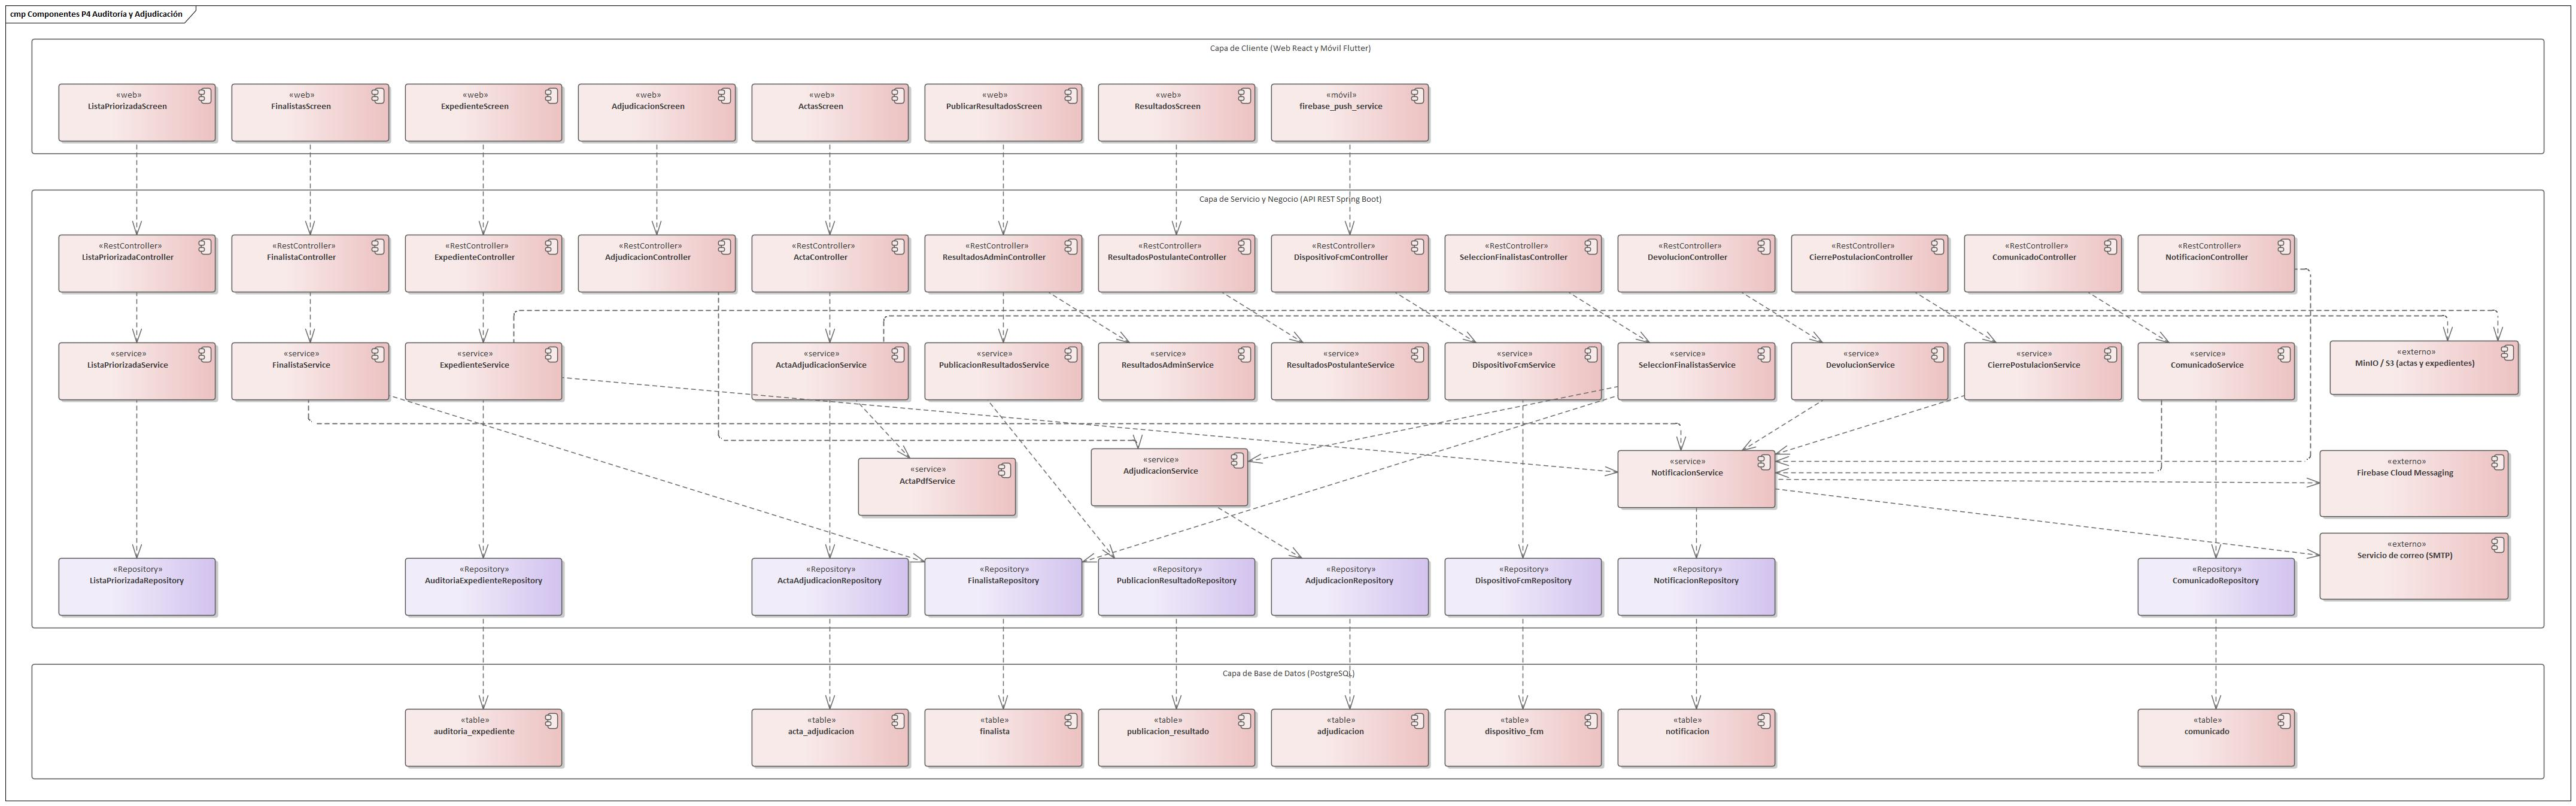
\includegraphics[width=\linewidth,height=0.8\textheight,keepaspectratio]{images/151_Componentes_P4_Auditoria_y_Adjudicacion.jpg}

\smallskip
\noindent\raggedright\textit{Nota.} Elaboración propia.
\end{figure}
\end{landscape}


\wfb{\wn{8}.2.5. Implementación de la Arquitectura del Subsistema Becados y Asistencia}\label{sec:cap8_sub_p5}

Este subsistema agrupa los casos de uso CU23, CU09, CU10, CU11, CU24.

Administra el padrón de becados (alta, baja, suspensión y reemplazo), genera las planillas de asistencia en PDF, registra la asistencia digital desde la app móvil del personal del comedor, coteja el registro contra el respaldo físico y permite al becado consultar su historial de asistencia y el estado de su beca.

La Figura~\ref{fig:impl_p5} presenta el diagrama de componentes del subsistema. Sus componentes son los siguientes:

\begin{itemize}
\item \textbf{Cliente web:} \texttt{PadronScreen}, \texttt{PlanillasScreen}, \texttt{CotejoScreen}, \texttt{MiBecaScreen}.
\item \textbf{Cliente móvil:} \texttt{registrar\_asistencia\_screen}, \texttt{mibeca (mi\_beca\_vista)}.
\item \textbf{Controladores:} \texttt{PadronController}, \texttt{BecaController}, \texttt{PlanillaController}, \texttt{AsistenciaController}, \texttt{CotejoController}, \texttt{MiBecaController}.
\item \textbf{Servicios:} \texttt{PadronService}, \texttt{BecaEstadoService}, \texttt{PlanillaAsistenciaService}, \texttt{PlanillaPdfService}, \texttt{AsistenciaService}, \texttt{CotejoAsistenciaService}, \texttt{MiBecaService}.
\item \textbf{Repositorios:} \texttt{BecaRepository}, \texttt{MovimientoBecaRepository}, \texttt{PlanillaAsistenciaRepository}, \texttt{AsistenciaRepository}, \texttt{CotejoAsistenciaRepository}, \texttt{MiBecaConsultaRepository}.
\item \textbf{Tablas:} \texttt{beca}, \texttt{movimiento\_beca}, \texttt{planilla\_asistencia}, \texttt{asistencia}, \texttt{cotejo\_asistencia}.
\item \textbf{Componentes externos:} MinIO (planillas PDF).
\end{itemize}

\begin{landscape}
\begin{figure}[p]
\caption{Diagrama de Componentes de la Implementación de la Arquitectura del Subsistema Becados y Asistencia}
\label{fig:impl_p5}
\centering
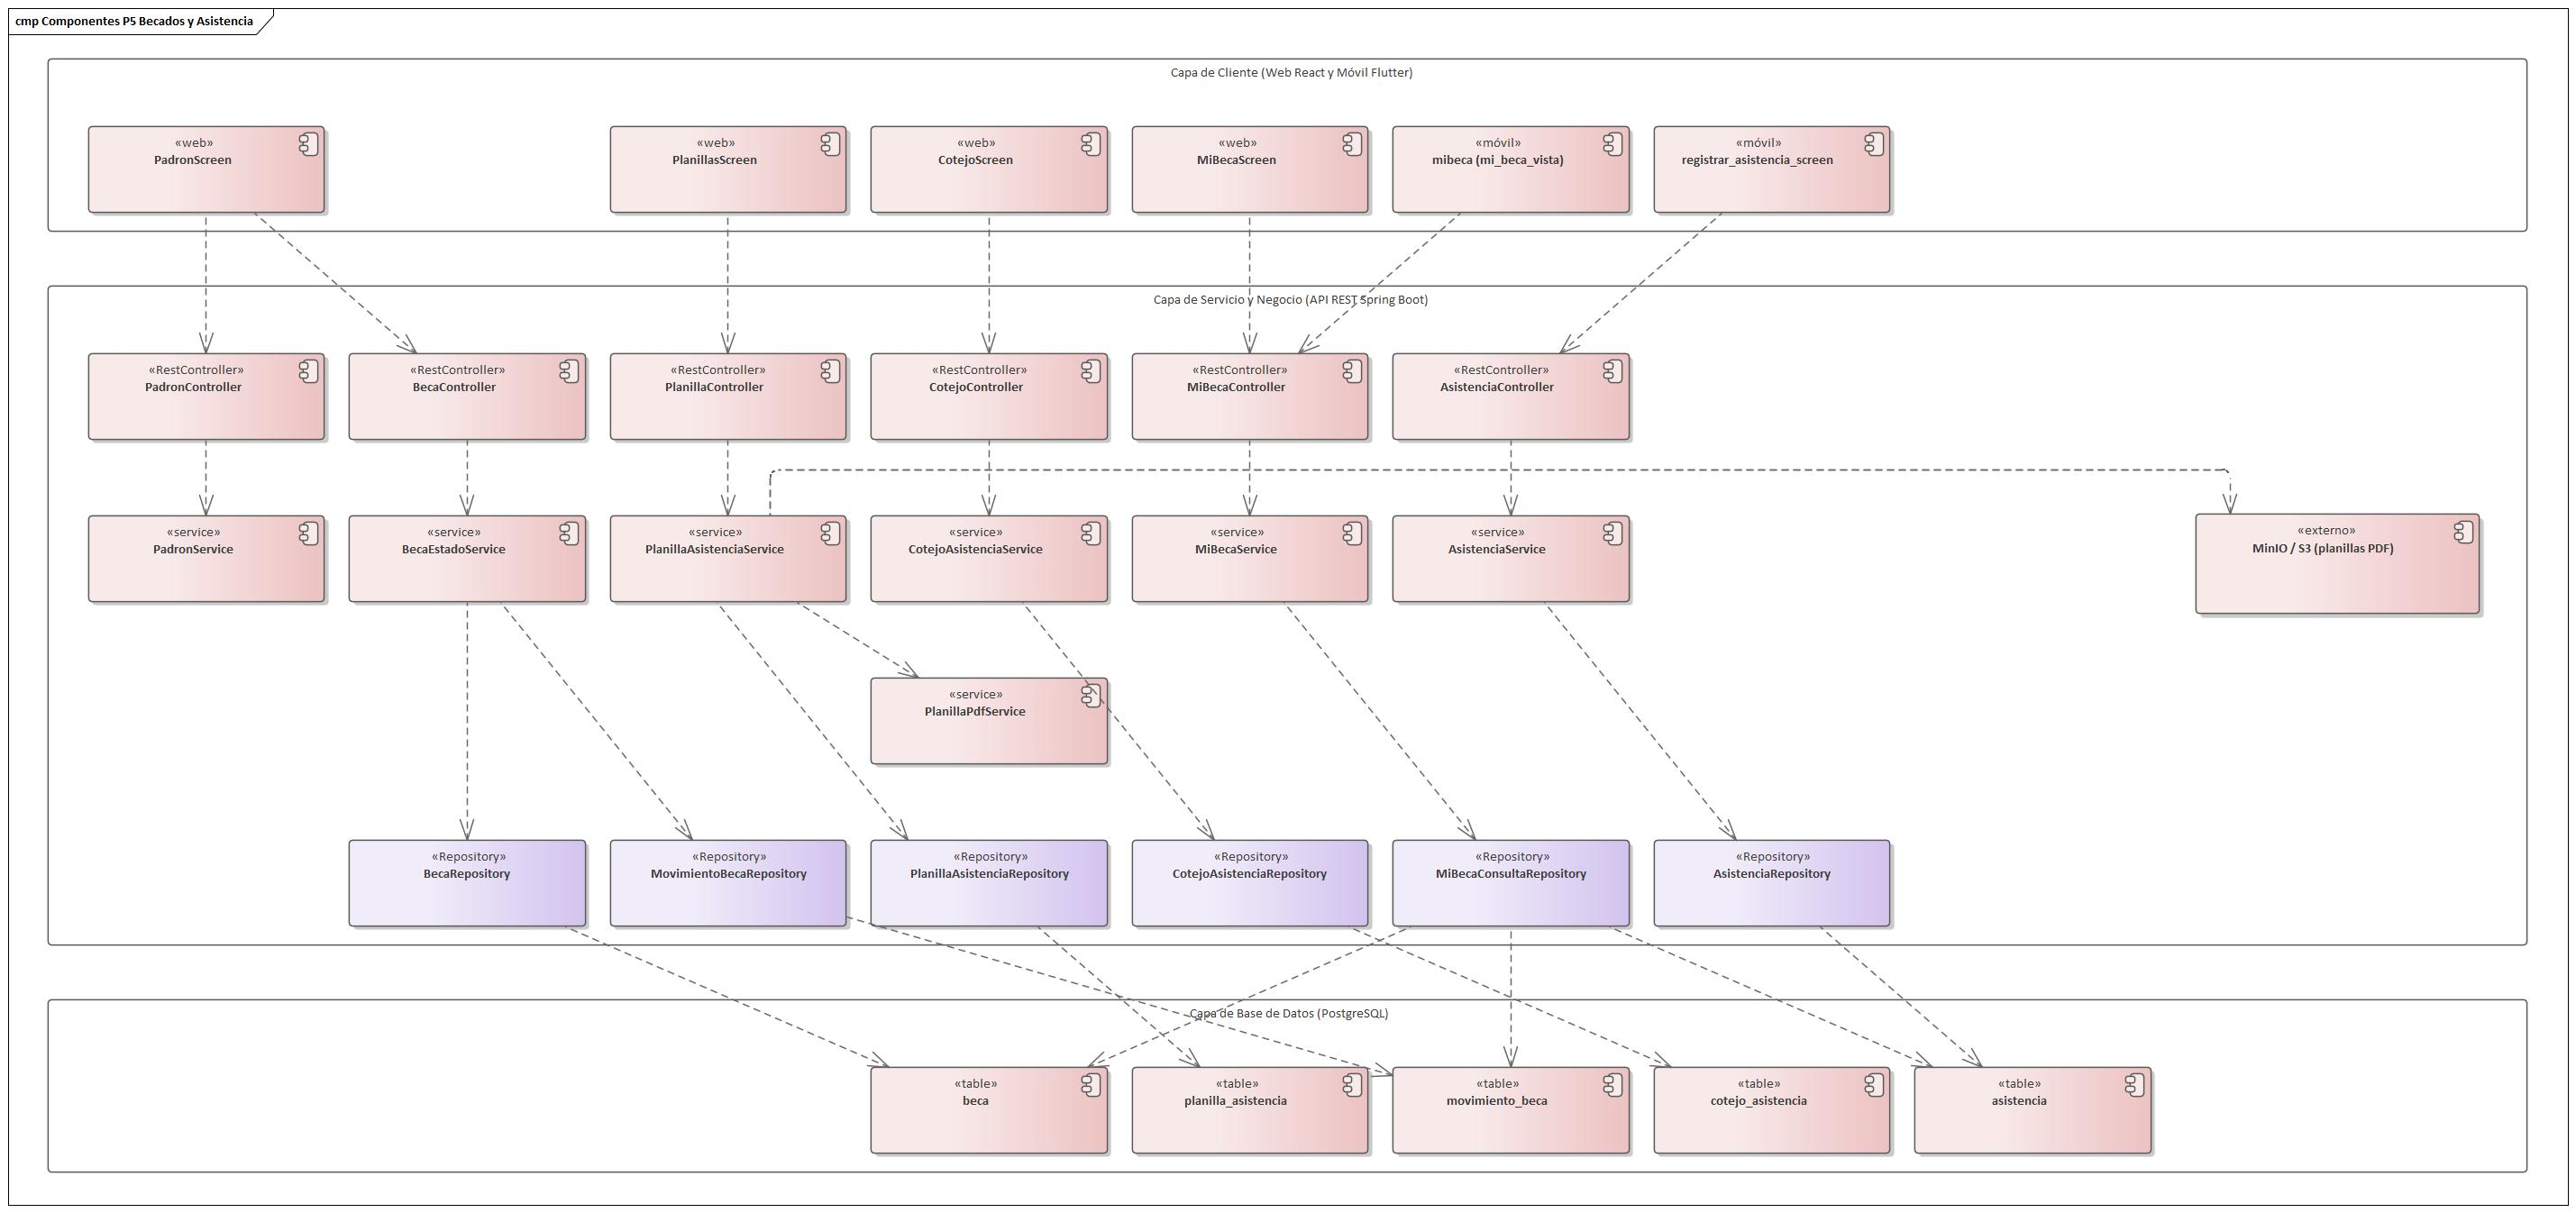
\includegraphics[width=\linewidth,height=0.8\textheight,keepaspectratio]{images/152_Componentes_P5_Becados_y_Asistencia.jpg}

\smallskip
\noindent\raggedright\textit{Nota.} Elaboración propia.
\end{figure}
\end{landscape}


\wfb{\wn{8}.2.6. Implementación de la Arquitectura del Subsistema Reportes y Trazabilidad}\label{sec:cap8_sub_p6}

Este subsistema agrupa los casos de uso CU12, CU25.

Ofrece el tablero de indicadores BI para el directivo (con exportación a Excel y PDF y caché en Redis), la bitácora de acciones del sistema y los paneles de inicio por rol. Los indicadores se leen de cinco vistas materializadas de PostgreSQL que \texttt{RefrescoIndicadoresJob} y \texttt{RefrescoIndicadoresService} actualizan; la bitácora se escribe desde cualquier servicio mediante la anotación \texttt{@Auditar} (\texttt{AuditoriaAspect}).

La Figura~\ref{fig:impl_p6} presenta el diagrama de componentes del subsistema. Sus componentes son los siguientes:

\begin{itemize}
\item \textbf{Cliente web:} \texttt{DashboardScreen}, \texttt{BitacoraScreen}, \texttt{PanelAdministradorScreen}.
\item \textbf{Controladores:} \texttt{DashboardController}, \texttt{BitacoraController}, \texttt{PanelController}.
\item \textbf{Servicios:} \texttt{IndicadoresService}, \texttt{BiService}, \texttt{FiltrosDashboardService}, \texttt{BiExcelService}, \texttt{IndicadoresPdfService}, \texttt{RefrescoIndicadoresJob}, \texttt{BitacoraService}, \texttt{BitacoraConsultaService}, \texttt{PanelService}.
\item \textbf{Repositorios:} \texttt{IndicadoresRepository}, \texttt{BiRepository}, \texttt{FiltrosDashboardRepository}, \texttt{BitacoraRepository}, \texttt{PanelRepository}.
\item \textbf{Tablas:} \texttt{mv\_bi\_asistencia\_dia}, \texttt{mv\_indicadores\_convocatoria}, \texttt{mv\_bi\_carrera\_convocatoria}, \texttt{mv\_bi\_convocatoria}, \texttt{mv\_bi\_puntaje\_convocatoria}, \texttt{bitacora}.
\item \textbf{Componentes externos:} Redis (caché del dashboard BI, CU12).
\end{itemize}

\begin{landscape}
\begin{figure}[p]
\caption{Diagrama de Componentes de la Implementación de la Arquitectura del Subsistema Reportes y Trazabilidad}
\label{fig:impl_p6}
\centering
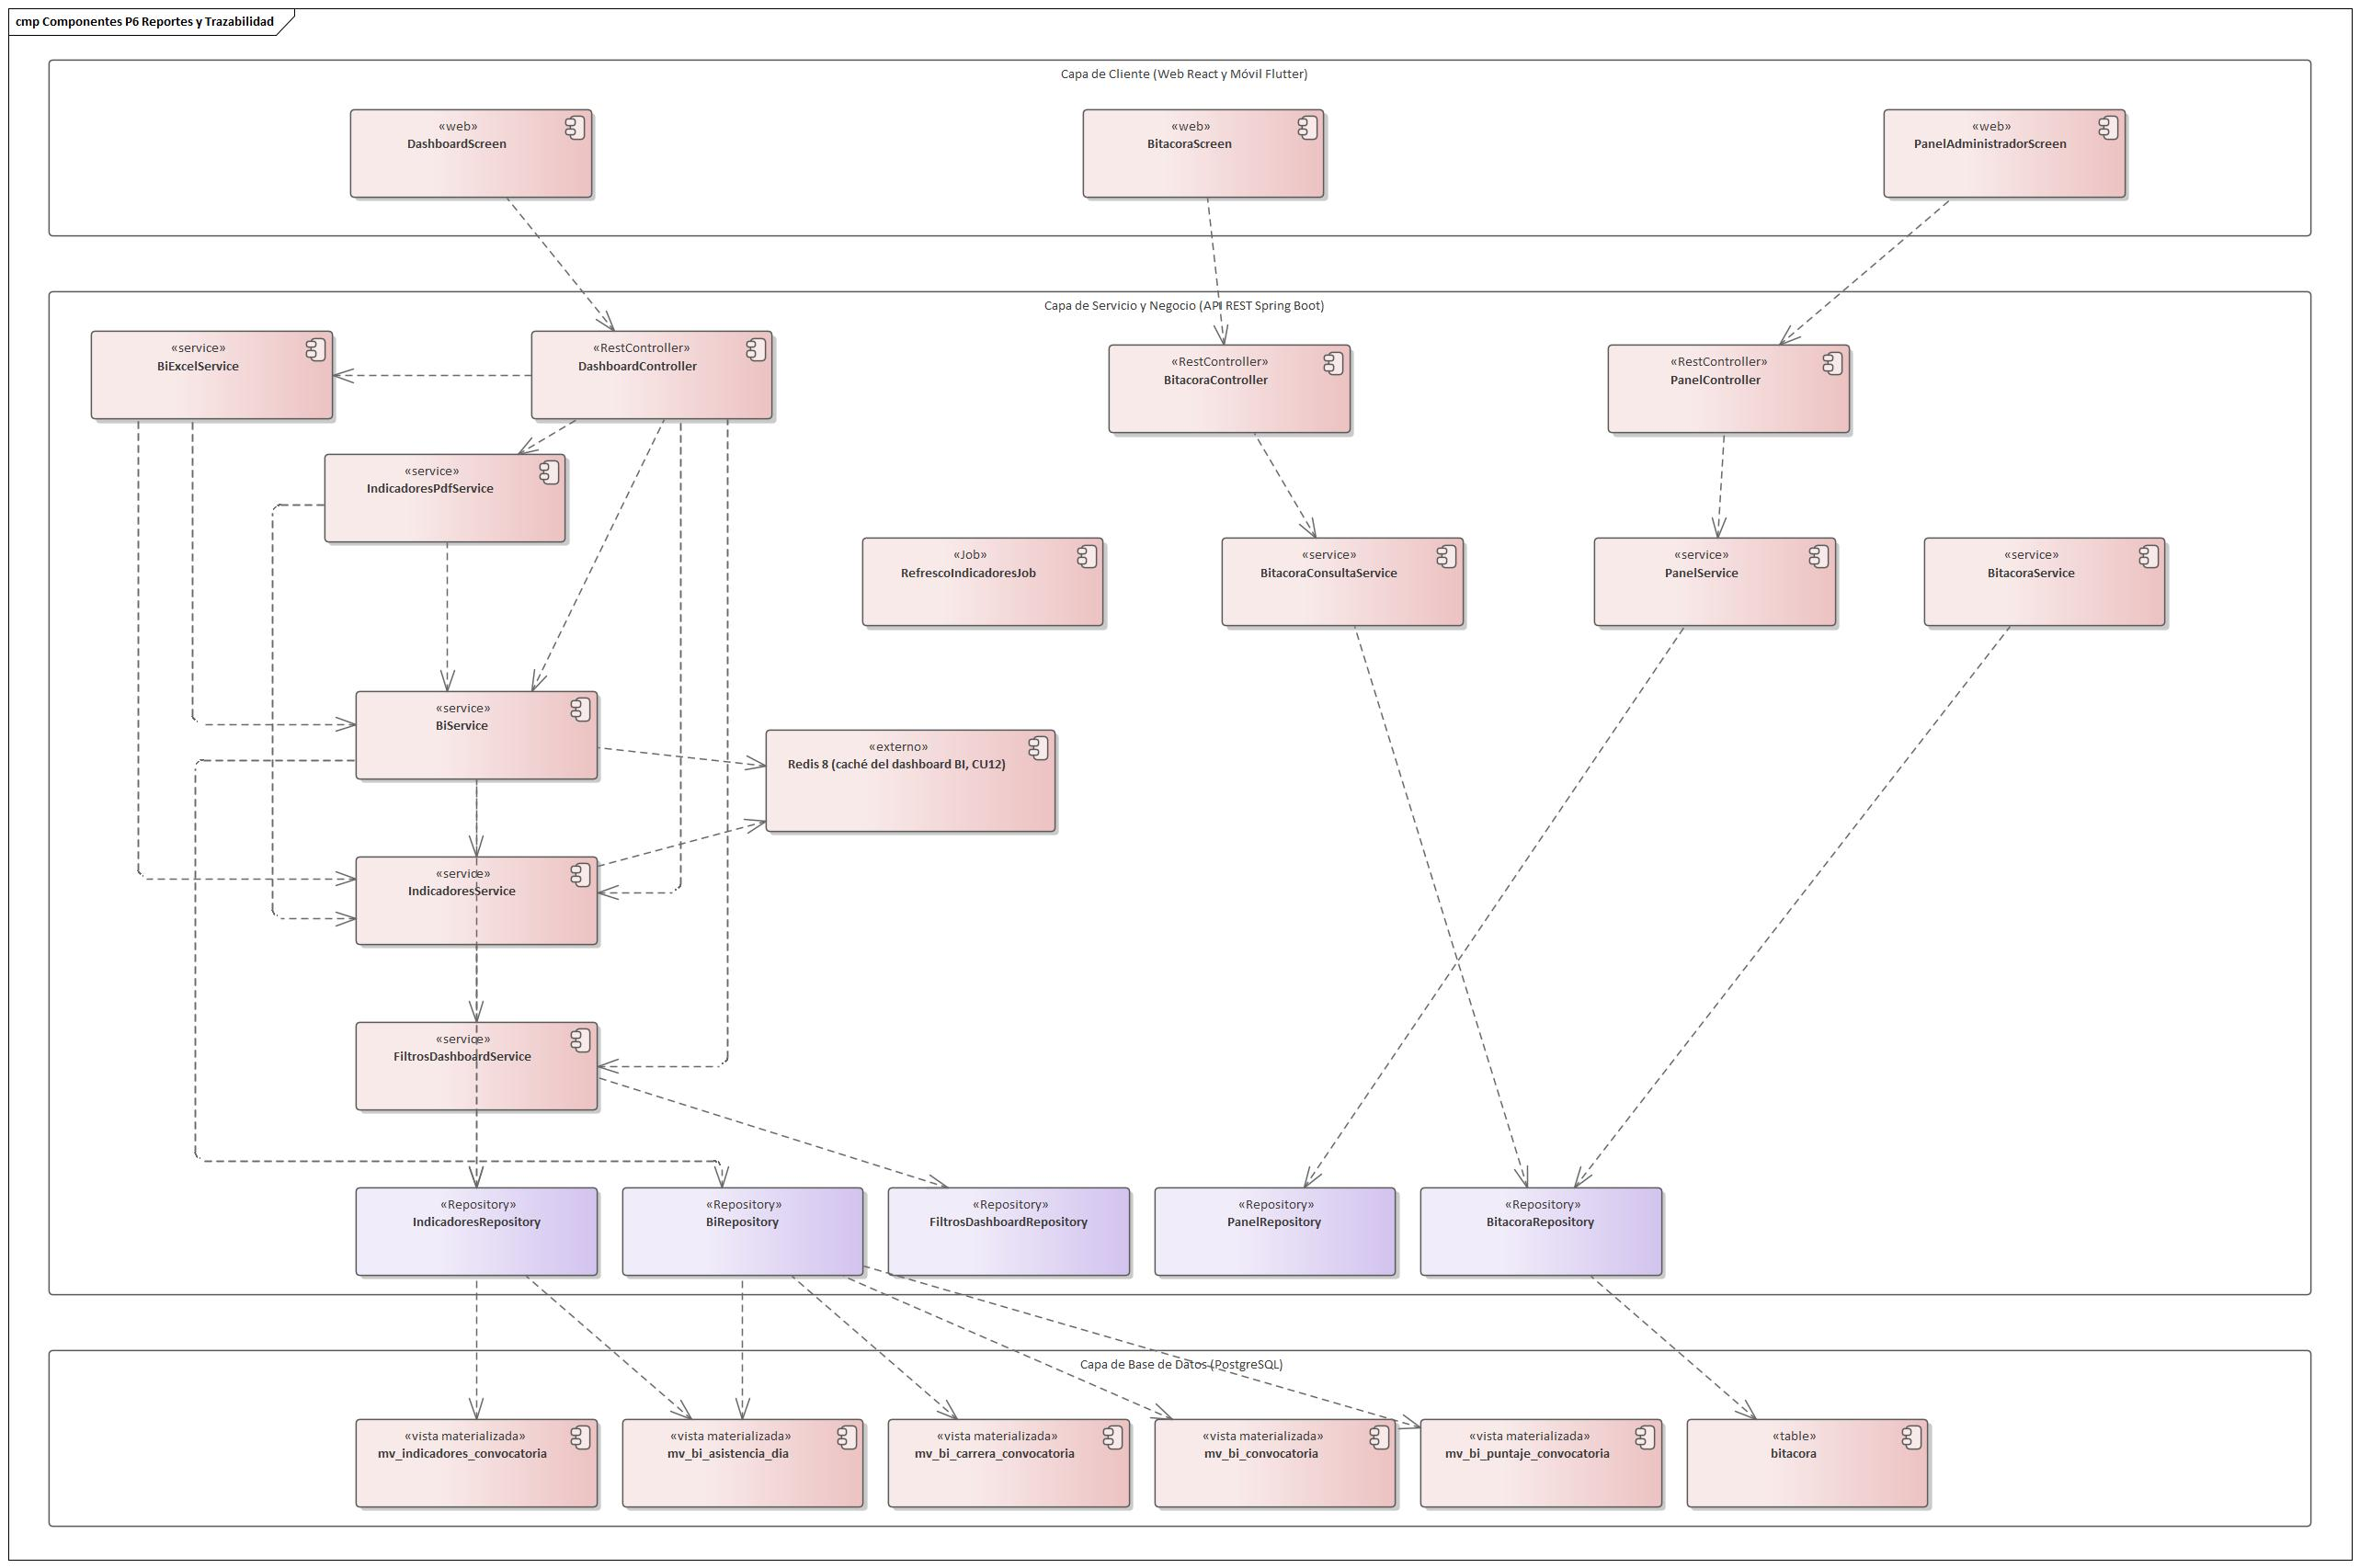
\includegraphics[width=\linewidth,height=0.8\textheight,keepaspectratio]{images/153_Componentes_P6_Reportes_y_Trazabilidad.jpg}

\smallskip
\noindent\raggedright\textit{Nota.} Elaboración propia.
\end{figure}
\end{landscape}

